\subsection{Résultats}

En raison de la date avancée du rendu du rapport de stage par rapport à la fin de mon stage, prévue pour le 27 août, les résultats présentés dans la section suivante sont basés sur l'état d'avancement jusqu'à présent. Veuillez noter que les résultats définitifs peuvent différer de ceux décrits ici.

\subsubsection{L'API}

L'API que j'ai développée permet actuellement d'effectuer des opérations CRUD (Create, Read, Update, Delete) sur différentes entités clés de l'application, notamment :

\begin{itemize}
	\item L'entité "Association", qui stocke des informations sur les différentes associations de l'école ainsi que les événements qu'elles ont créés.
	
	\item L'entité "Event", qui contient des informations détaillées sur un événement spécifique.
	
	\item L'entité "PeriodicEvent", qui modélise les événements périodiques sous forme de listes d'événements.
	
	\item L'entité "Registration", qui enregistre la participation d'un étudiant à un événement.
	
	\item L'entité "User", qui stocke les données liées aux utilisateurs.
\end{itemize}

En plus des opérations CRUD, l'API inclut d'autres fonctionnalités telles que la vérification de l'inscription de l'utilisateur à la fois dans le serveur Keycloak et dans la base de données.

\medskip

À ce stade, la majeure partie des fonctionnalités prévues a été mise en place. Des améliorations mineures pourraient être apportées d'ici la fin du stage, mais les bases de l'API resteront globalement inchangées. D'autres fonctionnalités, telles qu'un système de balises (tags) et la gestion des paiements pour les événements, sont prévues pour une mise en œuvre ultérieure au cours de l'année.

\subsection{L'application web}

L'application web que j'ai développée propose actuellement plusieurs onglets permettant d'interagir avec l'API de manière conviviale. La page d'accueil offre une vue d'ensemble de tous les événements créés par les associations (voir la figure \ref{fig:homepage}). À partir de cette page, les utilisateurs ont la possibilité d'accéder aux détails d'un événement, de s'inscrire à celui-ci ou de suivre une association. Un deuxième onglet permet d'afficher les événements des associations auxquelles l'utilisateur est abonné.


Une autre page est dédiée à la création d'événements (voir la figure \ref{fig:createevent}). Cette fonctionnalité est réservée aux membres autorisés de chaque association. Les événements sont hautement personnalisables et peuvent être configurés comme ponctuels ou périodiques.


En outre, une page spéciale permet aux administrateurs de visualiser la liste des utilisateurs inscrits.

\medskip

L'application a été conçue pour fonctionner de manière fluide à la fois sur les téléphones mobiles et sur les ordinateurs, grâce à la philosophie du développement "mobile-first". En suivant cette approche, l'application est initialement conçue en mettant l'accent sur l'expérience utilisateur mobile, puis les éléments peuvent être progressivement ajoutés pour s'adapter aux écrans d'ordinateurs tout en préservant la convivialité mobile.

\medskip

Quelques ajustements restent à apporter à l'application web d'ici la fin du stage, notamment~:

\begin{itemize}
	\item  La création d'une page d'administration facilitant les opérations CRUD sur la base de données.
	
	\item L'ajout d'une page utilisateur pour consulter les événements auxquels l'utilisateur est inscrit.
	
	\item La conception d'une page spéciale pour les créateurs d'événements, où ils pourront consulter la liste des étudiants inscrits à leurs événements.
	
	\item Un changement dans le style de la page est prévu afin qu'elle corresponde davantage à l'identité de l'association et qu'elle ne paraisse pas comme une application dépourvue de personnalité.
\end{itemize}

\begin{figure}[!h]
	\centering
	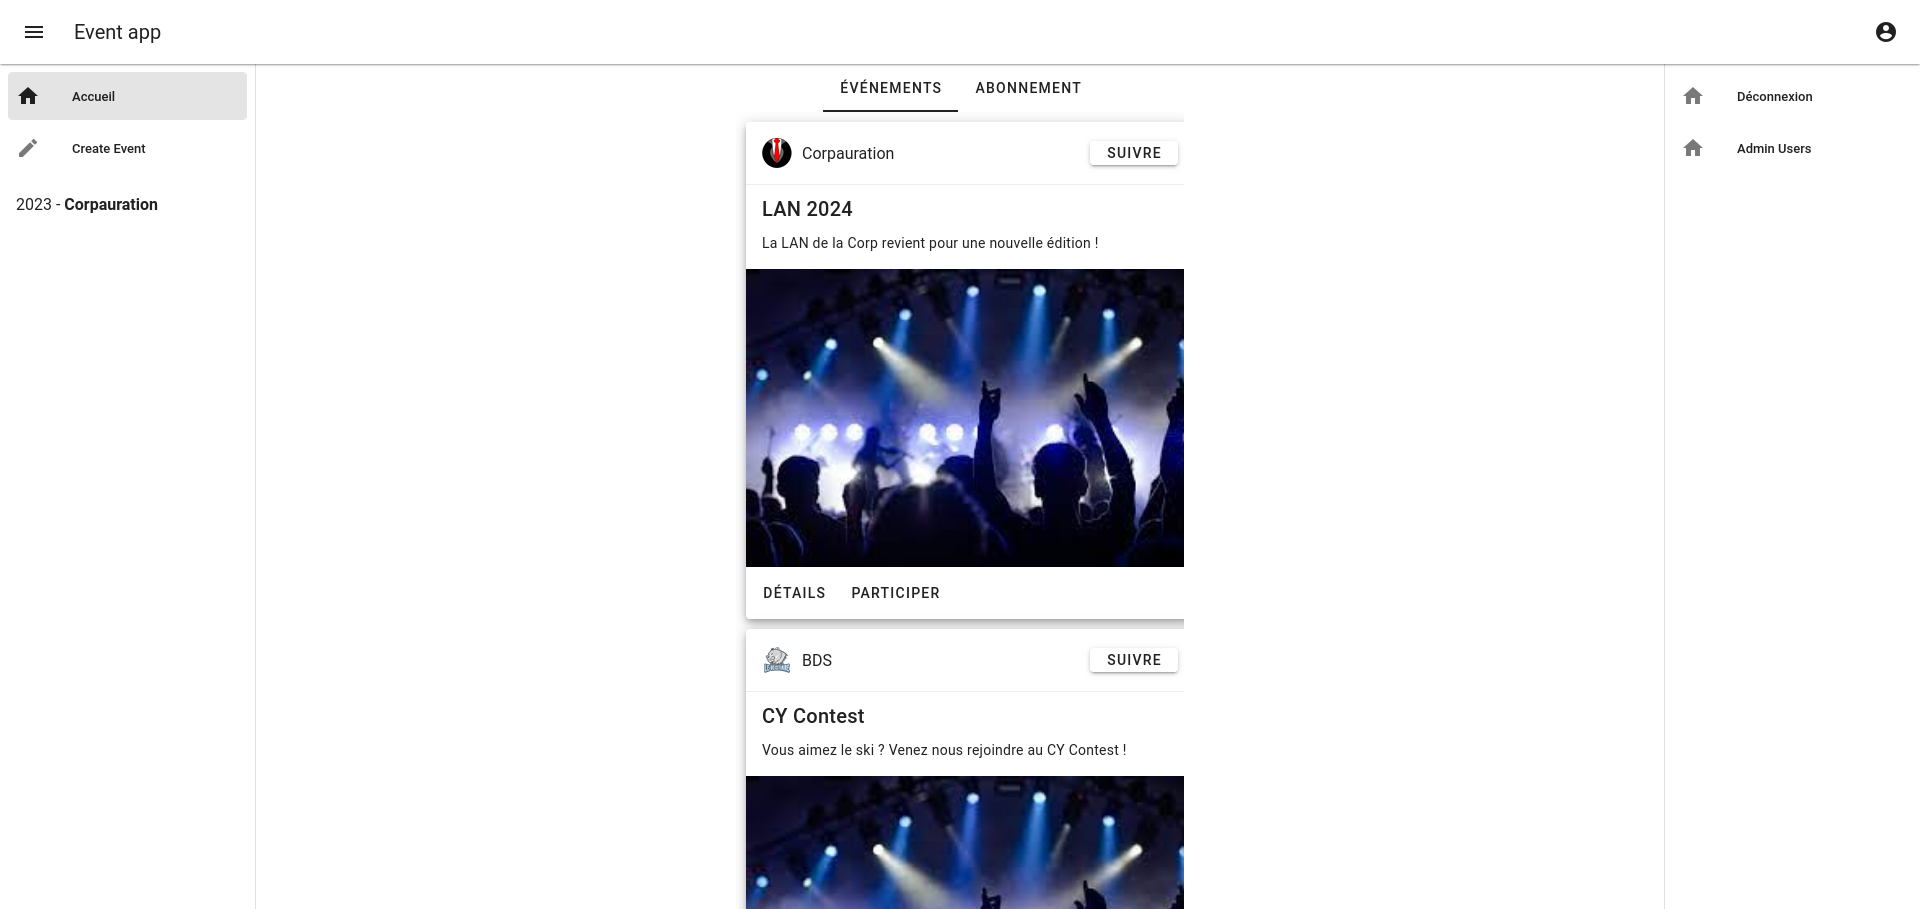
\includegraphics[width=0.95\textwidth]{assets/homepage.png}
	\caption{Page d'accueil}
	\label{fig:homepage}
\end{figure}


\begin{figure}[!h]
	\centering
	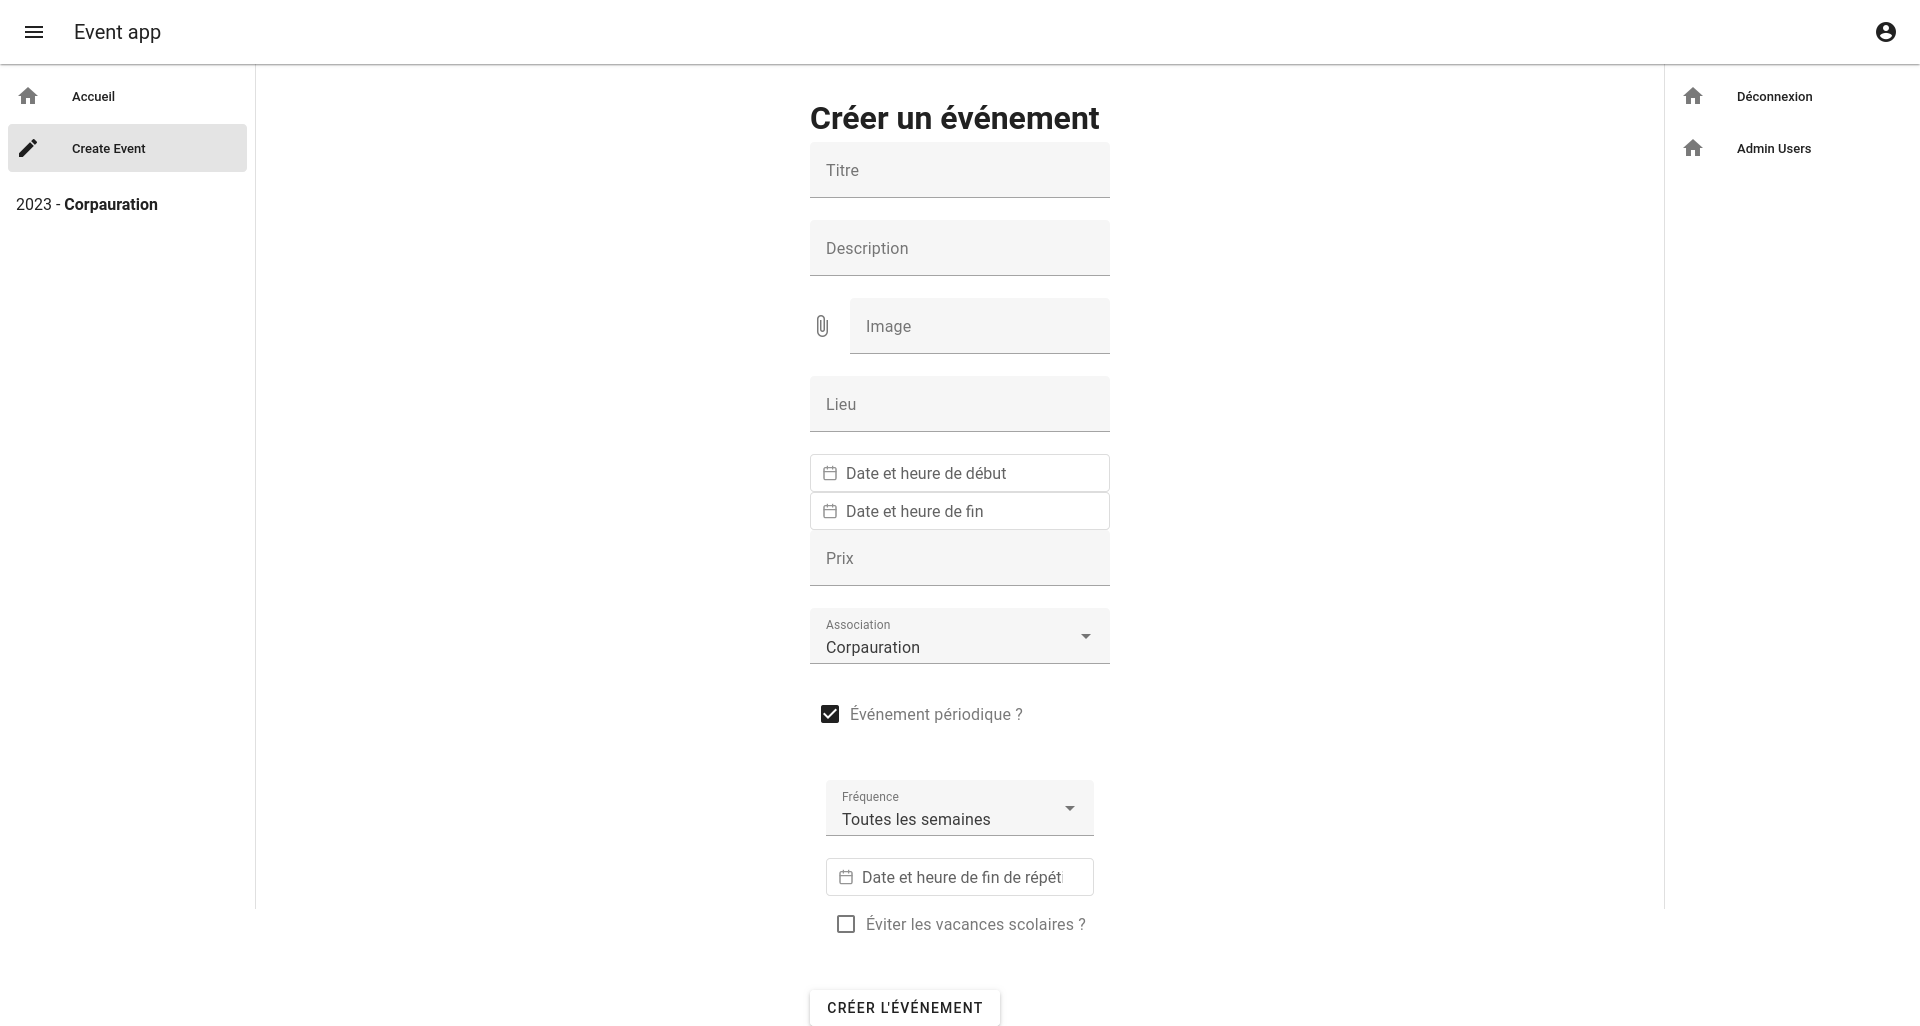
\includegraphics[width=0.95\textwidth]{assets/createevent.png}
	\caption{Page de création d'événements}
	\label{fig:createevent}
\end{figure}